\section{Pāli Phonetics and Pronunciation}
\label{phonetics}

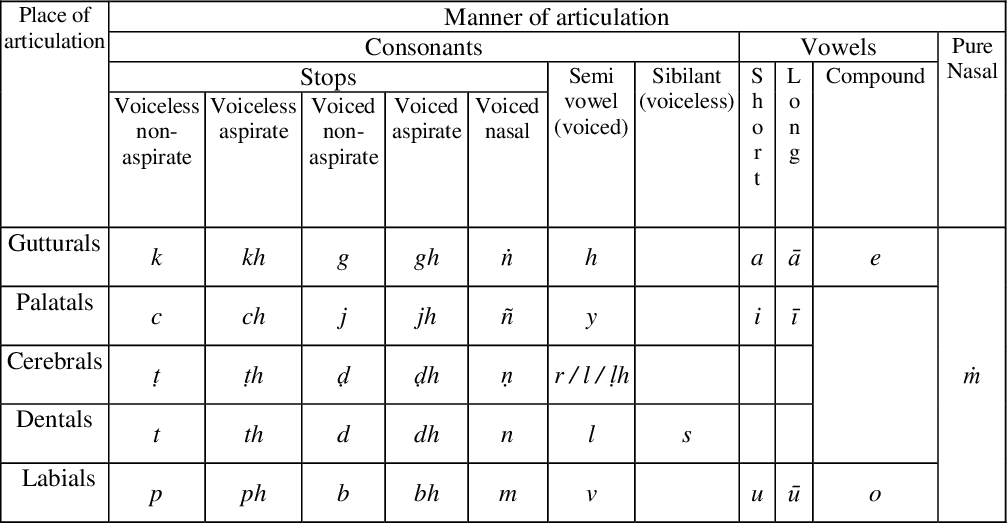
\includegraphics[width=\textwidth]{pali-table.png}

\begin{justify}
Pāli is the original scriptural language of Theravāda Buddhism. It was a spoken language, closely related to Sanskrit, with no written script of its own. As written forms have emerged, they have been in the letterings of other languages (e.g. Devanagari, Sinhalese, Burmese, Khmer, Thai, Roman). The Roman lettering used here is pronounced as in English, with the following clarifications:
\end{justify}

\medskip

% TODO works but must be a way to split both boxes evenly
\textbf{Vowels} are of two types:\\
\begin{minipage}{.55\textwidth}
  \begin{tabular}{@{} ll @{}}
    \textbf{Short} & \textbf{Long}\\
    \textbf{a} as in magm\prul{a} & \textbf{ā} as in f\prul{a}ther\\
    \textbf{i} as in l\prul{i}ter & \textbf{ī} as in mach\prul{i}ne\\
    \textbf{u} as in p\prul{u}t   & \textbf{ū} as in r\prul{u}le\\
                   & \textbf{e} as in \prul{e}nd\\
                   & \textbf{o} as in m\prul{o}re\\
  \end{tabular}
\end{minipage}% This must go next to `\end{minipage}`
\begin{minipage}{.453\textwidth}
  Exceptions: e and o change to short sounds in syllables ending in double consonants. They are then pronounced as in ``pet'' and ``soft'' respectively. (eg. sotthi)
\end{minipage}

\begin{justify}
\textbf{Consonants} are mostly as one would expect, with a few additional rules: Two-lettered notations with \textbf{h} (e.g. \textbf{kh}, \textbf{ch}, \textbf{ṭh}, \textbf{th}, \textbf{ph}) denote an aspirated, airy sound, and should be considered as one unit. They are distinct from the hard, crisp sound of a single consonant (e.g. \textbf{k}, \textbf{c}, \textbf{ṭ}, \textbf{t}, \textbf{p}). However, other combinations with \textbf{h}, i.e., \textbf{lh}, \textbf{mh}, \textbf{ñh}, and \textbf{vh}, do count as two consonants (e.g. `jivhā'or `muḷho').  Examples: \textbf{th} as t in tongue. (never pronounced as in ``the'') \textbf{ph} as p in palate (never pronounced as in ``photo'').
\end{justify}

\begin{justify}
These are distinct from the hard, crisp sound of the single consonant, e.g. th as in ``Thomas'' (not as in ``thin'') or ph as in ``puff'' (not as in ``phone'').
\end{justify}

\textbf{ḍ} , \textbf{ḍh} , \textbf{ḷ} , \textbf{ṇ} , \textbf{ṭ} , \textbf{ṭh}

\begin{justify}
These retroflex consonants have no English equivalents. They are formed by curling the tip of the tongue back against the palate.
\end{justify}

\textbf{Miscellaneous}
\begin{justify}
The semivowel ``\textbf{v}'' is pronounced as in ``\textbf{w}e'' ``\textbf{ñ}'' is pronounced as in ``ca\textbf{ny}on'' The pure nasal ``\textbf{ṁ}'' and voiced nasal ``\textbf{ṅ}'' are pronounced as in ``su\textbf{ng}''.
\end{justify}

\begin{justify}
As an aid to understanding, \textbf{hyphens} (-) have often been inserted in longer Pāli compounds, in order to indicate the separate words that make up the compound. This should not affect the pronunciation during recitation in any way. In order to not suggest unintended pauses in the flow of the recitation, punctuation marks (commas, periods, colons and semicolons) were removed for most chants. \textbf{Line breaks} within a sentence indicate that a short breathing pause is inserted, but indented line breaks indicate that recitation continues without a breathing pause.
\end{justify}

\begin{justify}
Elsewhere, \textbf{breath marks} ( \breathmark\ ) have been inserted in order to indicate breathing pauses. When reciting as a group, each participant is encouraged to recite as accurately, audibly, and continuously as within one's capabilities; ideally from the first chant to the last without interruption, gaps, or omissions. However, passages within \textbf{brackets }[…] serve as an introduction, and are recited only by the leader. Except for Pāli paritta and funeral chants, there is a pause after […], before the rest of the group joins in.
\end{justify}

\clearpage
